\documentclass{article}

\usepackage{graphicx}
\usepackage{wrapfig}
\usepackage{multirow}
\usepackage{url}

\newcommand{\db}{\textsf{VMGdB}}

\title{\db\\the CONTACT Visuo Motor Grasping dataBase}

\author{N. Noceti \and C. Castellini \and B. Caputo \and G. Sandini \and F. Odone}

\begin{document}

\maketitle

\begin{abstract}

 Grasping is one of the most interesting challenges in nowadays robotics, posing
 problems to the mechanical and electronic engineer, the computer vision researcher,
 the control theorist and, more recently, the neuroscientist. The study
 of human grasping has proved beneficial to get a better understanding of the problem.
 In this paper we present \db, the CONTACT Visuo-Motor Grasping Database, a recording
 of grasping actions performed by $20$ human subjects on $7$ objects using $5$ ways of
 grasping, under variable illumination conditions. The \db\ consists of $5200$ grasping
 acts organized in $260$ data entries --- each of which made of $2$ video sequences
 recorded from two colour cameras, and motor data recorded from a sensorised glove.
 Labeled data are available as standard AVI videos and a file of ASCII outputs from the glove.
 %Ground truth is available for all samples in the database.
%\textbf{Claudio: a cosa ti riferisci? CC: al fatto che il db contiene la label di ogni singolo sample.}
 The \db\ provides to the community a reliable and flexible testbed for tackling the
 problem of grasping from a humanoid/human-oriented perspective, and hopefully not
 only that.

\end{abstract}

\section{Introduction}

Grasping is a serious challenge to nowadays robotics. As research moves towards
more and more unstructured environments, the characteristics of the objects to
be grasped (shape, texture, weight) become unpredictable; the illumination and
colour conditions of the scene must be taken into account; and, as better and
better grippers/hands are available, the kinematics and dynamics of the
end-effector must enter the picture, too. As an example, consider a rover equipped
with a hand-arm system intended to pick up samples of Martian rocks and soil, and
to then drop them in the correct test tube: such a system must be able to grasp
with a so-far unprecedented ability.

A recent trend to solve this problem (to which so far no general solution is known)
draws inspiration from human grasping and its developmental nature. This is in the
first place inspired by the amazing ability of humans to grasp; for instance Gibson's
re-definition of objects in terms of affordances \cite{gibson1,gibson2}
entails that the way an object can be grasped is essential to its model, which can
then be used in a robotic artifact. More recently, this idea has been boosted by
the discovery of a neural correlate to affordances, namely mirror neurons and
mirror structures, both in high primates and humans
\cite{gallese-96,umilta-01,rizzolatti-04,friston09}. If this paradigm is correct,
then studying human grasping is paramount for good robotic grasping.

Starting from this working hypothesis, we hereby present to the community
\db, the CONTACT Visuo-Motor dataBase, obtained by recording (both in video
and with a dataglove) $5200$ grasping acts, performed by $20$ human subjects on
$7$ different objects and with $5$ different grasp types.

\subsection{Motivation and aims}

The intentionally unstructured illumination conditions, and the fact that the
objects are of the most diverse shapes, textures and colours, make this database
a rather realistic ground model of the human act of grasping. Two different
points of view and the use of a magnetic tracker plus a dataglove, ensure that
we have a clear representation of the action. The fact that the \db\ collects
such diverse data as far as the subjects/objects/grasps are concerned makes it
suited, for instance,

\begin{itemize}

\item to model and understand the act of grasping itself (prediction of the hand
      final position and posture, detection of the preshaping phase, classification
      of the type of grasp, etc.);

\item to enrich the visual model of objects, adding the knowledge of the type of
      grasp employed for each object;

\item if a task-related prior is given, to then choose an appropriate robotic
      grasp; and so on.

\end{itemize}

Even though grasping is being extensively studied, as far as we know
this is the first publicly available database aimed at the study of grasping as a
dynamic act. Interesting similar, but not comparable, attempts appear in the
GRASP project \cite{grasp_project}, where a highly detailed taxonomy of grasp
types is described, and in the Columbia Grasp Database \cite{GoldfederAl09}, which
consists of synthetic grasps generated using a simulator.

The \db\ follows the idea described in \cite{lopes-05,metta-06} and
it represents an extension and an advancement of it, both in a
qualitative and quantitative sense.

\subsection{Paper structure}

The paper is organized as follows. Section 2 details the acquisition protocol,
describing the how the acquisition setup and the experiments were designed, 
Section 3 illustrates the dataset and additional material included to the \db,
and Section 4 is left to the conclusions. 

\section{The acquisition protocol}

This section sketches the main elements of the acquisition system and details
on the acquisition experimental procedure.

\subsection{Setup}

The acquisition setup was designed in order to give an accurate and meaningful
representation of the act of grasping an object by the volunteers. Its main
components are two colour cameras for the visual representation; and 
a magnetic tracker, a virtual-reality sensorised glove and a pressure sensor
for the haptic/motor representation. All devices are connected to a standard
biprocessor desktop computer equipped with a hard disk large enough to contain
all required data, and fast enough not to loose any data while recording. 

Human subjects would sit on a comfortable chair in front of a desk onto which %to
an object would be placed; the subject was asked to grasp the object with his/her
right hand while wearing the glove, and then to put it back in the original position
on the table with the left hand, as the right hand goes back to the resting position.
Therefore, a full grasping act goes from the hand resting position, to the grasping
instant and then back to the resting position.

The desk is uniformly dark green and non-reflective; the objects were chosen
to be colourful; and the illumination was provided by two windows looming over
the desk. Intentionally we did not fix the illumination condition (that changed
over time since acquisition sessions spanned over a week), now and then fixing
the white balance of the cameras in order to avoid saturation.

%Figure \ref{fig:setup} is a picture of the setup.
%
%\begin{figure}[ht]
%  \centering
%  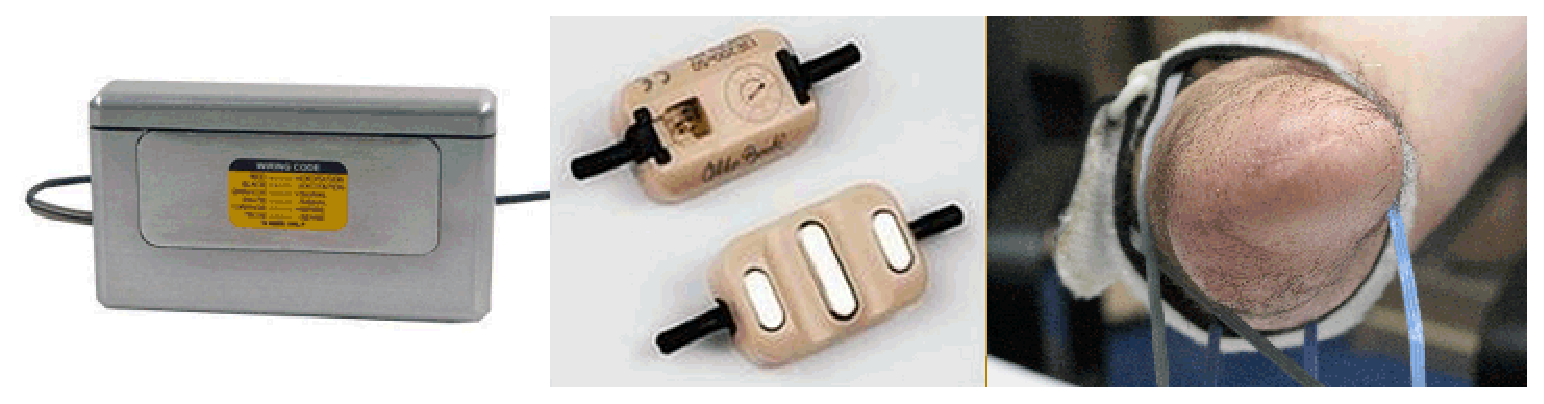
\includegraphics[width=.5\textwidth]{images/setup}
%  \caption{view of the setup with a subject.}
%  \label{fig:setup}
%\end{figure}

The cameras are Watec \emph{WAT-202D} colour cameras, operating at $25$Hz and
connected to two Picolo PCI-bus frame grabbers. One camera
was placed in front of the subject while the other was placed on the right-hand side
of the subject, almost framing the object in a close-up and focussed upon it. The
first camera has the view of what an external observer would be seeing of the grasp;
the second would give an accurate representation of the act of grasping in full detail,
including the last moments of the reaching sequence.

The subjects would wear a $22$-sensors Immersion \emph{CyberGlove}
\cite{cyberglove} right-hand sided dataglove,
which provides $22$ $8$-bit numbers linearly related to the
angles of the subject's hand joints. The resolution of the sensors is on average about
$0.5$ degree. The sensors describe the position of the three phalanxes of each finger
(for the thumb, rotation and two phalanxes), the four finger-to-finger abductions,
the palm arch, the wrist pitch and the wrist yaw. The magnetic tracker was an
Ascension \emph{Flock-Of-Birds} \cite{fob} mounted on the subject's wrist, which
would return six real numbers, the linear and angular coordinates of the wrist
with respect to a base mounted on the far end of the desk. Lastly, a standard force
sensing resistor (FSR) glued to the subject's thumb was used to determine the
instant of contact with the object.

\subsection{Experiment design}

The dataset is built considering 7 different objects ((see Fig. \ref{fig::grasps}), top)
and 5 grasps ((see Fig. \ref{fig::grasps}), bottom). The objects have been selected to
represent different materials, colors and shapes, and to them we associate a set of
appropriate grasps \cite{grasp_project}: each object can be grasped, in general, in
many different ways, according to the many-to-many relationship reported in Table
\ref{tab:manytomany}. In total $13$ {\em (grasp,object)} pairs are considered, according
to everyday experience.

\begin{table} \centering
 \label{tab:manytomany}
 \caption{The $13$ {\em (grasp,object)} pairs in the \db. Each grasp is performed
          on the related object $20$ times by each of the $20$ subjects,
          resulting in $5200$ grasping acts. Boldface {\bf X}s are the pairs
          visibile in Figure \ref{fig::grasps}, bottom row.}
 \begin{tabular}{c||c|c|c|c|c|c|c} \hline
                   & ball    &     pen &  duck   &     pig &  hammer & tape & lego brick \\ \hline\hline 
   cylindric power &         &         &         & {\bf X} &         &      &            \\ \hline
              flat &         &         &         &         & {\bf X} &      &     X      \\ \hline
             pinch &         & {\bf X} &    X    &         &         &   X  &     X      \\ \hline
         spherical & {\bf X} &         &         &         &         &   X  &            \\ \hline
          tripodal &    X    &       X & {\bf X} &         &         &   X  &            \\
 \end{tabular}
\end{table}

\begin{figure}[!ht]
	\centering
	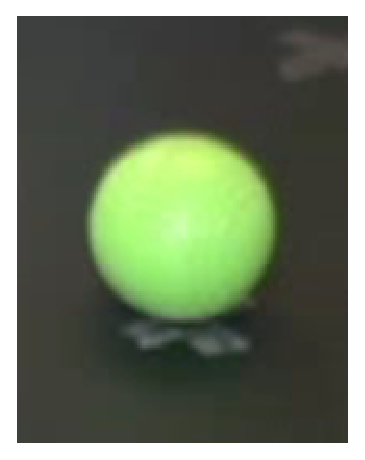
\includegraphics[height=1.75cm]{images/palla}
	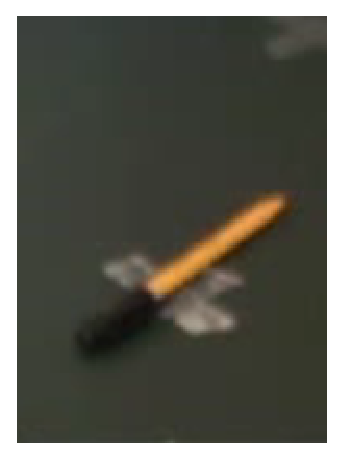
\includegraphics[height=1.75cm]{images/penna}
	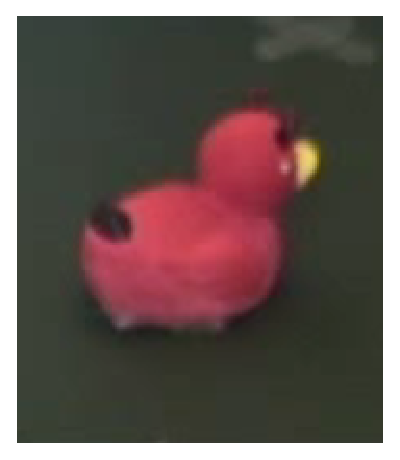
\includegraphics[height=1.75cm]{images/papera}
	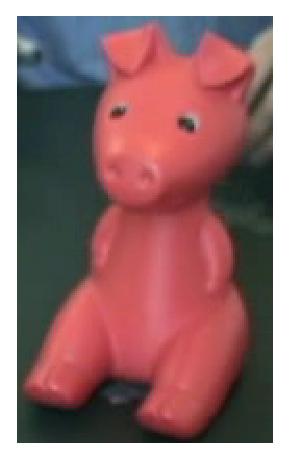
\includegraphics[height=1.75cm]{images/porcellino}
	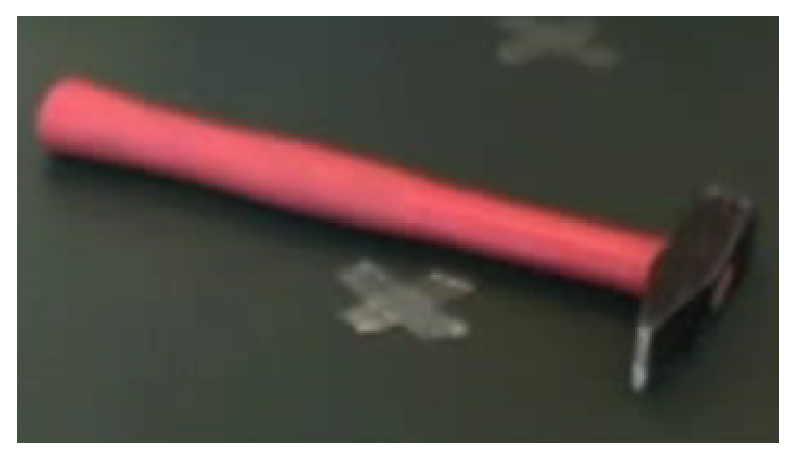
\includegraphics[height=1.75cm]{images/martello}
	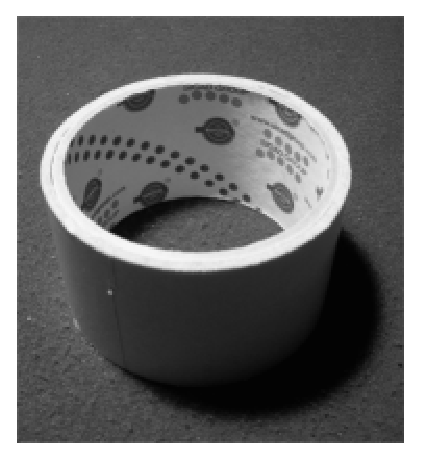
\includegraphics[height=1.75cm]{images/scotch}
	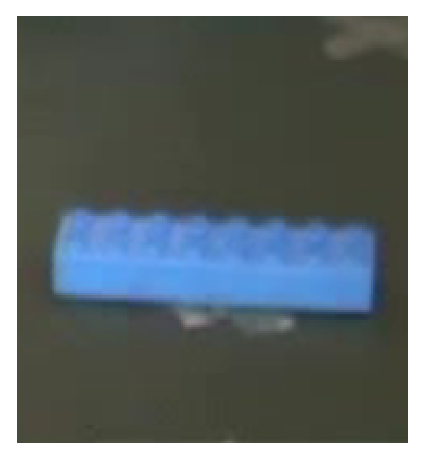
\includegraphics[height=1.75cm]{images/lego}\\
	\vskip 0.1cm
	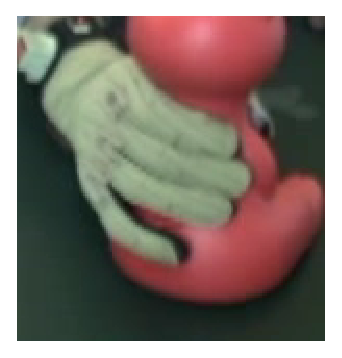
\includegraphics[width=0.19\textwidth]{images/cylinder}
	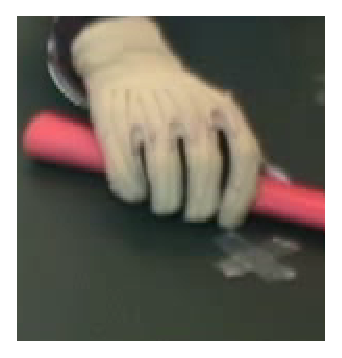
\includegraphics[width=0.19\textwidth]{images/flat}
	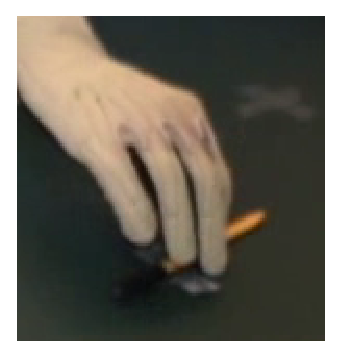
\includegraphics[width=0.19\textwidth]{images/pinch}
	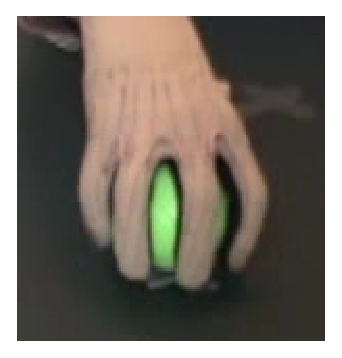
\includegraphics[width=0.19\textwidth]{images/spherical}
	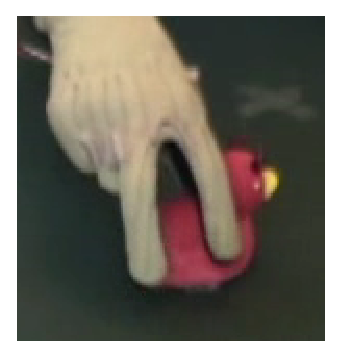
\includegraphics[width=0.19\textwidth]{images/tripodal}
	\caption{{\em (top row)} The $7$ objects in the \db.
         {\em (bottom row)} The $5$ grasp types in the \db\ (left to right: cylindric power
         grasp, flat, pinch grip, spherical and tripodal grip) applied to five
         of the considered objects.}
	\label{fig::grasps}
\end{figure}

The subjects pool includes $20$ right-handed people, $6$ females and $14$ males,
aged between $24$ and $42$ years (mean $31.5$ years, median $31$).
%The volunteers (computer scientists, mathematicians, physicists, and engineers from our
%research labs)  are  2 senior researchers, 8 post-docs, 7 phd students, 3 undergraduate students.
Each of the $260$ {\em (subject,object,grasp)} triplets is an entry of the database;
each entry was performed $20$ times, giving a total of $5200$ grasping acts.

The next section describes in details the available data for each experiment.

\section{The \db}

In this section we report the structure of the \db, with a comment on the
peculiarities of the data and a brief description on the data annotation features.

\subsection{Data}

Each of the $260$ {\em (subject, object, grasp)} entries is associated to the following data: 

\begin{itemize}

 \item {\bf Visual information.} Two video sequences ($384 \times 288$ $25$ fps
   AVI, MPEG-4 compression, YV12 colorspace) acquired by the two cameras with a
   focus on the object and on the action respectively. The videos report the whole
   grasping action, from a hand rest position to the final grasp and then back.
   Figure \ref{fig::grasp_sequence} shows sample frames from the two sequences.
   Each video sequence is associated to a data file (ASCII format) mapping
   single video frames to the acquisition time-stamp, allowing for synchronization
   with the sensor data.

 \item {\bf Hand posture sensor information.} One file (ASCII format) containing
   information from the sensor glove as the grasping action occurs as well as the
   acquisition time-stamp (Table \ref{tab:motordata} lists in details the content
   of each row of the file). The latter is used for synchronization with the visual data.

\end{itemize}		

Both videos and ASCII files contain all information related to a whole
{\em (subject, object, grasp)} experiment, i.e., to $20$ consecutive 
grasping actions performed by the same subject on a given object-grasp pair.

\begin{figure}[!ht]
	\centering
	\includegraphics[height=1.75cm]{images/frontal1}
	\includegraphics[height=1.75cm]{images/frontal2}
	\includegraphics[height=1.75cm]{images/frontal3}
	\includegraphics[height=1.75cm]{images/frontal4}
	\includegraphics[height=1.75cm]{images/frontal5}\\
	\vskip 0.1cm
	\includegraphics[width=0.19\textwidth]{images/side1}
	\includegraphics[width=0.19\textwidth]{images/side2}
	\includegraphics[width=0.19\textwidth]{images/side3}
	\includegraphics[width=0.19\textwidth]{images/side4}
	\includegraphics[width=0.19\textwidth]{images/side5}
	\caption{Synchronized sample frames from the two video sequences, showing
	  the evolution of the grasping action (from the hand rest position to
	  object lifting and then back to rest). }
	\label{fig::grasp_sequence}
\end{figure}

\begin{table} \centering
 \label{tab:motordata}
 \caption{Items contained in each row of the sensor data file.}
 \begin{tabular}{|l|l|l|}
   \hline 
   {\bf $\#$} &     {\bf data type} & {\bf comments}                       \\
   \hline 
            1 &             real & time stamp (starting from $0$)       \\
            6 &             real & measurements from the Flock-of-Birds \\
           22 &  $8$-bit integer & measurements from the Cyberglove     \\
            1 & $16-bit$ integer & measurement from the pressure sensor \\
   \hline
 \end{tabular}
\end{table}

\subsection{Additional material}

Together with the data described above, supplemental material is made
available to increase the database usability.

{\bf Object visual appearance.} A set of $20$ plain images of each object
depicted in the acquisition environment is included as additional material. 
A crop of these images to contain the sole object region is also available.

{\bf Synchronization.} The two video sequences have been acquired at $25$Hz by each camera, while the glove,
magnetic tracker and pressure sensor have been sampled at $100$Hz. Since the three
devices are independent of one another, a time-stamp is associated to each numerical
sample and frame (for each of the cameras) in order to reconstruct the exact time
sequence of data and to obtain a full synchronization of visual and sensorial information.
A script associating each sensor datum the corresponding video frames is available; because of the different acquisition frequency of the different
devices there will not be, in general, an exact correspondence between time-stamps. Thus the script implements a nearest
neighbor strategy to find the video-frames closest in time to the sensor datum.

{\bf Istantaneous visuo-motor data.} The database contains information on the whole grasp action, from the hand rest position and back. 
This can be useful to researchers wishing to
exploit the action evolution for what concerns visual or motion features, or both. In the case instantaneous information on the actual grasping 
is needed we included a script 
which extracts static visual and motion features from the dynamic data sequences. When
applied to a ({\em subject, object, grasp}) experiment, it extracts the 20 image frames  and an ASCII file with the 20 vector measurements of the joints 
corresponding to the 20 grasps within this experiment.

The grasping instant is estimated by locating extrema  from the pressure sensor.
Figure \ref{fig::pressureplot} reports the values of the pressure sensor positioned on the thumb (first of the 4 pressure values), along an experiment. The zoomed plot shows
in details a single action from one rest position to the next rest position. 

\begin{figure}
	\begin{center}
	\includegraphics[height=10cm]{images/pressure_plot.pdf}
	\caption{A plot of the thumb pressure sensor values used to estimate the 20 grasping instants within one experiments. The zoom shows in details a single action.}
	\label{fig::pressureplot}
	\end{center}
\end{figure}

\subsection{Data peculiarities}
The data have been acquired under loosely controlled conditions. As mentioned in Section 2.1, during acquisition the scene was illuminated 
by natural light with a significant illumination change from sequence to sequence. 

Also, the subjects  were encouraged to act ``naturally", 
therefore there is a certain variability in the way actions were performed. For most subjects, it is also noticeable a speed increase as the experiments
proceed and the actor gets familiar with the experimental protocol. 

All these features make the visual data very close to natural acquisition settings and give raise to typical issues of an artificial vision system ---  
non uniform illumination, shadows, occlusions, just to name a few (see Figure \ref{fig::light_variations}). For these reasons the \db\  is an ideal test-bed for validating
solutions to be then applied to the real world.

\begin{figure}[!ht]
	\centering
	\includegraphics[height=2.1cm]{images/light1}
	\includegraphics[height=2.1cm]{images/light2}
	\includegraphics[height=2.1cm]{images/light3}\\
	\includegraphics[height=2.1cm]{images/lightB1}
	\includegraphics[height=2.1cm]{images/lightB2}
	\caption{$3$ frontal (top) and $2$ lateral (bottom) sample frames of the
	  same nature extracted from different experiments, showing the variability
	  of illumination conditions and, consequently, the varying amount of shadows.}
	\label{fig::light_variations}
\end{figure}

\section{Conclusions}

The CONTACT Visuo-Motor Grasping Database, \db, has been presented in this paper.
It consists of a large collection of synchronised video sequences and sensor
data acquired by a sensorized glove, faithfully representing the act of human grasping. 

The data was obtained with the help of $20$ human subjects engaged in grasping $7$
common objects in $5$ different ways. In total, there are $260$ experiment entries,
recording $5200$ grasping actions. The acquisition setting was intentionally loosely
controlled, thus visual appearance may change due to variable illumination, shadows
and occlusions caused by the actors hands. For these reasons the \db\ represents a
rather challenging set of data, ideal to depict common problems of an artificial
vision environment. 

Along with visuo-motor dynamic data, recording the whole grasping sequence, the
\db\ includes images of the plain objects and a script to extract instantaneous static
information (both visual and sensorial) on the precise instant when grasping occurs.
This feature would make the database useful to researcher not wishing to exploit the
full grasping dynamics. 

The \db\ is publicly available at ... \textbf{CLAUDIO SAYS: qui dobbiamo decidere COME renderlo pubblico.}
{\bf FRA: proporrei una semplice pagina web con materiale da downloadare, un readme file semplice e questo papiro, quando ci sara' piu' eventuali lavori correlati.
Una cosa cosi': http://www.bioid.com/downloads/facedb/index.php o anche piu' semplice. Sul "dove" il nostro sito e' attualmente in fase di aggiornamento ma nel caso saremo felici di ospitare il db. Altrimenti IDIAP?
CC: non posso che approvare!}.

\subsubsection*{Acknowledgements}

The authors are grateful to the twenty volunteers that participated to the acquisition sessions.
The work here described was partially supported by the EU-funded projects NEURObotics (FP6-IST-1917)
and Contact (NEST-5010). We also thank Giorgio Metta and Giulio Sandini of IIT, Genova, Italy,
for an early discussion about the experiment this database is based upon.

\bibliographystyle{alpha}
\bibliography{paper}

\end{document}
